\documentclass{article}
\usepackage{../acad} % https://github.com/rstanuwijaya/latex-template

\renewcommand{\sectionPrefix}{}

\title{PHYS5120 HW3}
\author{TANUWIJAYA, Randy Stefan \footnote{\LaTeX\ source code: \url{https://github.com/rstanuwijaya/hkust-computational-material/}}\\ (20582731) \\ rstanuwijaya@connect.ust.hk}
\affil{Department of Physics - HKUST}
\date{\today}

\begin{document}
	\maketitle
	\begin{section}{Monte Carlo (MC) simulations of Lennard-Jones Argon}
		Use the Metropolis Monte Carlo method to calculate the radial distribution function (RDF) in the homework 2. Discuss how to choose a good trial displacement. Is the RDF obtained by MC consistent with the one from MD? Which method is more efficient according to your experience? Why?
		\begin{tcolorbox}[breakable]
			The implementation of the Metropolis Monte Carlo method to calculate the radial distribution function (RDF) is attached separately. Here is the pseudocode for the Metropolis Monte Carlo method:

			\begin{algorithm}[H]
				\SetKwFunction{simulationStep}{simulationStep}
				\caption{Calculating RDF with MC method}
				\label{alg:MCsimulation}
				$N \leftarrow 0$ accumulator for accepted MC\;
				$M \leftarrow $ number of simulation steps\;
				$pos \leftarrow (N \times 3)$ FCC vector lattice in reduced unit\;
				$pot \leftarrow$ Potential energy of $pos$ using VdW potential in reduced unit\; 
				
				\While{pot is not converged}{
					$pos, pot, accepted \leftarrow \simulationStep{pos, pot}$\;
				}
				\For{$i < M$}{
					$pos, pot, accepted \leftarrow \simulationStep{pos, pot}$\;
					add relative $pos$ of each atom in minimum image convention to the RDF histogram\;
					$N \leftarrow N + accepted$\;
				}

				Print the ratio of accepted MC steps to total MC steps $\eta \leftarrow N/M$\;
				Plot the RDF histogram for $r < L_{box}/2$\;
			\end{algorithm}

			Where the simulation step function is given in Algorithm \ref{alg:simulationStep}.

			\begin{algorithm}[H]
				\SetKwFunction{simulationStep}{simulationStep}
				\SetKwProg{Fn}{Function}{}{}
				\caption{Simulation Step Function for MC method}
				\label{alg:simulationStep}
				\Fn{\simulationStep{pos, pot}}{
					$prop\_pos \leftarrow pos + \Delta (Rand(0,1) - 0.5)$\;
					$prop\_pot \leftarrow$ Potential energy of $prop\_pos$ using VdW potential\;
					$acc = \min\left( 1, \exp\left( -(prop\_pot - pot)/(T_0) \right) \right)$\;
					$accepted \leftarrow Rand(0,1) < acc$\;
					\If{accepted}{
						$pos \leftarrow prop\_pos$\;
						$pot \leftarrow prop\_pot$\;
					}
					\Else{
						$pos \leftarrow pos$\;
						$pot \leftarrow pot$\;
					}
					\Return pos, pot, int(accepted)
				}
			\end{algorithm}
			Where $T_0$ is the system temperature in reduced unit.

			Below is the result of the RDF using $M = 8000$ simulation steps for $N\_cell = \{3, 4, 5\}$.

			\begin{figure}[H]
				\centering
				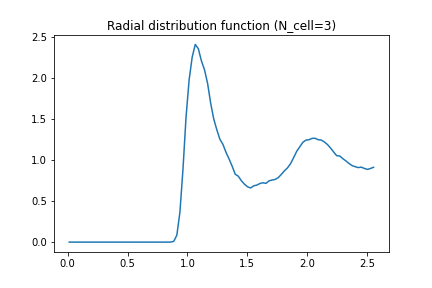
\includegraphics[width=0.8\textwidth]{./images/g_r(N_cell=3).png}
				\caption{RDF from MC method $(N\_cell=3)$}
				\label{fig:RDF_MC3}
			\end{figure}

			\begin{figure}[H]
				\centering
				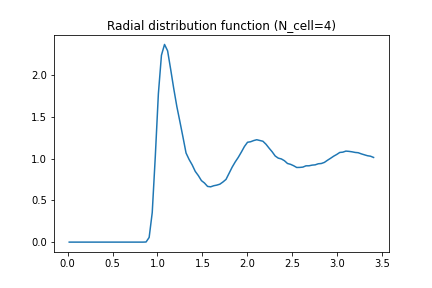
\includegraphics[width=0.8\textwidth]{./images/g_r(N_cell=4).png}
				\caption{RDF from MC method $(N\_cell=4)$}
				\label{fig:RDF_MC4}
			\end{figure}

			\begin{figure}[H]
				\centering
				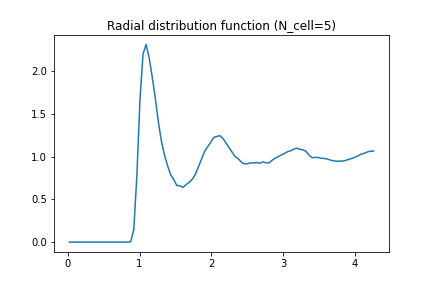
\includegraphics[width=0.8\textwidth]{./images/g_r(N_cell=5).png}
				\caption{RDF from MC method $(N\_cell=5)$}
				\label{fig:RDF_MC5}
			\end{figure}

			\newpage
			\begin{enumerate}
				\item To choose a good trial displacement, we need to choose a displacement that is small enough to avoid large energy changes, but large enough to avoid the system to be trapped in a local minimum. In this case, we can observe the value of $\eta = N/M$, i.e. the number of accepted MC steps divided by the total number of MC steps. For our trial, we choose $\Delta$ such that $\eta$ is around $0.15-0.3$.
				
				\item The RDF obtained by MC is consistent with the one from MD. The difference is that the RDF from MC is more noisy, but the overall shape is the same. 
				
				\item There are two considerations for deterimining the effiency of this method. 
				
				In terms of the physical process involved, MC method is more effiecent compared to MD method. This is because the MC method only needs to calculate the potential energy of the system, while the MD method needs to calculate the force of each atom. 
				
				On the other hand, in terms of the simulation time, MC method might needs longer time to converge to the equilibrium state. For example, our simulation uses ~16k MC steps to reach the equilibrium state, while the MD method only needs <1k steps. 
			\end{enumerate}
			\end{tcolorbox}
	\end{section}
\end{document}
